\section{System Model}\label{sec_system}
The system model shown in Figure \ref{fig_system} is captured as 5-tuple $\langle A,N,\mapsto,Req,Pro\rangle$, where \ttsexp{A}{A}[k] denotes software applications, \ttsexp{N}{n}  heterogenous computation (or computing nodes) $\mapsto: A\rightarrow N$ maps the software applications to at least a single computing node, and $Req, Pro$ are assignment functions, respectively defines the requirements of the applications and resource provisions of the computing nodes. The  function $Req:A\rightarrow (\mathrm{RL,EE,CL}):\mathbb{R}^+\times [0,1]\times \mathbb{I}^+$ a, assigns the reliability, end-to-end timing and criticality level of applications. The function $Pro:N\rightarrow (\mathrm{HZ,PW,FR}):\mathbb{R}^+\times \mathbb{R}^+\times \mathbb{R}^+$ assigns, respectively the processor speed, power consumption and failure rate of the computing nodes. 

The end-to-end timing requirements are the timing constraints over the end-to-end functional behaviors of the applications. These requirements are often specified on the \textit{cause-effect chains} consisting of software components and (potentially network messages) within the application. The reliability requirement is the expected reliability goal of an application which is discussed further in Subsection \ref{subsec_reliability_constraint}, and the criticality level signifies the importance of an application over other applications that have lower criticality levels, thus prioritizing the application during resource contention. The criticality levels are defined systematically, e.g., following the hazard analysis according to the ISO 26262 standard for functional safety in road vehicles~\cite{iso201126262}. 

%resource provisions of%contains of three parts: software applications, an execution platform, and an allocation scheme. In this section, we show models of the different parts and describe them in detail. For the sake of clarity, first we list the main mathematical notations that are used to define the system model and the software allocation problem.
 \begin{figure}[!h]
 \centering
 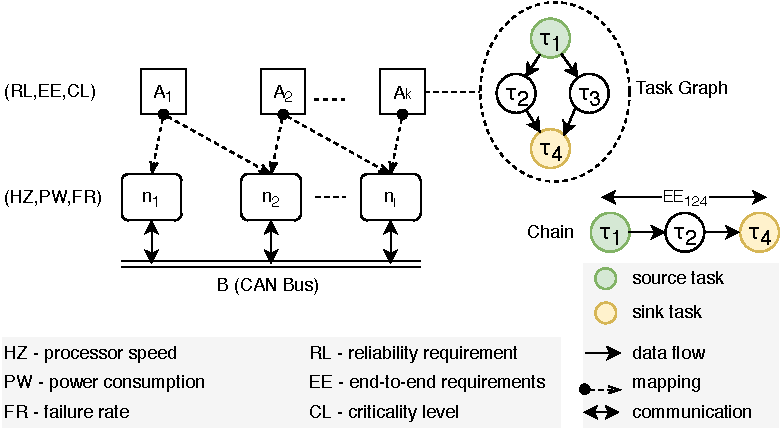
\includegraphics[scale=0.8]{system_model}%softwareallocation
 \caption{System Model.}
 \label{fig_system}
 \end{figure}
\begin{table}[]
	\small
\begin{tabular}{@{}llp{0.55\textwidth}@{}}
\toprule
 & Notation                        & Description                                             \\ 
\midrule
 &/* Application related */&\\
$\bullet$ & \ttsexp{A}{A}[k]     	            & software applications* \\
$\bullet$ & \multicolumn{2}{p{0.8\textwidth}}{$\sss{g}[k][]$  denotes the directed acyclic graph of $A_k$, where $V(g)$ is the set of node/vertices and $E(g)$ is the set of edges of $g$.}\\
$\bullet$ & \sexpsp{C}{c}     		             & software-component types of \ttssb{A}[k]**\\
$\bullet$ & \sexpss{Q}{q}    		            & component replicas of type \ttsss{c}\\
%$\bullet$ & \sexpss{R}[i]{r}[j]   	             & runnables that implement \ttsss{c}\\
%$\bullet$ & \sexpss{H}[i,j]{r}[h]              & runnables that implement $\sss{q}[k][i,j]$\\

&/* Execution platform related */ &\\
$\bullet$ & \ttsexp{N}{n}         	            & computation (or computing) nodes      \\
$\bullet$ & $B$         						           & shared CAN bus   \\
$\bullet$ & \ttsexp{M}{m}         	           & messages on the CAN bus   \\
$\bullet$ & \multicolumn{2}{p{0.8\textwidth}}{$\tau,c,m,\gamma$ denote iterator variables,  respectively for task, component, chain and node, e.g., $\forall \tau \in  \ssp{T}$.***}\\
 &/* Mapping related */&\\

$\bullet$ & \ttsexp{\textbf{x}}{\textbf{x}}[k]:$\bigcup{\sss{Q}}\mapsto M$            & a mapping vector from \ttssp{Q} to $M$             \\
$\bullet$ & \multicolumn{2}{p{0.8\textwidth}}{$k,i,j$ denote iterator index-variables,  respectively for the mapping vector \ttx, and rows and columns of the matrix \ttxsp{k}, e.g., \ttxkij.***}\\
$\bullet$ & $\sss{g}[k][\tau](\x)$   		           & directed acyclic graph of task nodes for $A_k$.\\
$\bullet$ & \sexpsp{\Gamma}{\Gamma}  & end-to-end chains             \\
$\bullet$ & \ttsss{\Gamma}$=(e_i)_{i=1}^Z$   & a chain of $e\in V(\sss{g}[k][\tau])\cup M$\\ 
&/* Functions related */ &\\

$\bullet$ & $Power(\textbf{x})$                		& total power consumption of  $A$ in \ttx    \\
$\bullet$ & $Reliability_{a}(\x)$      					& application reliability  of $a\in A$ in \ttx              \\
$\bullet$ & $ResponseTime_{\tau}(\x)$     		& response time of  $\tau \in V(\sss{g}[k][\tau])(\x)$                       \\
$\bullet$ & $Delay_\gamma(\x)$            			& age delay of $\gamma \in \ssp{\Gamma} $   in \ttx     \\
\bottomrule\\
\end{tabular}
{\footnotesize 
	*Note: the total elements in a set $S$ is denoted by \ttn{S}, e.g., \ttn{A} denotes the number of applications in the set $S$, essentially it refers to its cardinality.\\
	** For readability, we prefer to use \ttsss{S} in place of $\sss{S}[k]$. \\
   *** IFor other uses of the iterators, they are defined in the context.}
 
\end{table}

\subsection{Software Applications}
The software application represents an independent and self-contained user-defined software functionality, e.g., x-by-wire, electronic throttle control, flight control, etc. The application is assumed to be developed using the principles of model-based development and component-based software engineering~\cite{softwarecomponents}\cite{Crnkovic2002BuildingSystems}. 



%$\bigcup_{i=1}^{N_a} A_i$ 
\begin{definition}[Software Application Model]\label{def_application}
It is modeled as a set of communicating software components. Note that a software component is a design-time concept, representing the lowest-level hierarchical element in software architecture of the application. The set of software components in the application is modeled as a \textit{directed acyclic vertex-weighted} graph $\langle V_\tau,L_\tau, w\rangle$ of periodic task nodes $V_\tau$, where $a_{ij}\in L_\tau$ refers to the data-flow link from node $\tau_i$ to node $\tau_j$ and $i \neq j$. The function $w: V_\tau\rightarrow (e_{n_i},\mathrm{D,P})$ assigns computation cost to each task node, where  $e_m$ is worst-case execution tim (WCET) on the computing node $n_i$, D deadline and P period.
\end{definition}

Multiple applications can be executed on the same computating node(s) and can share the on-board network, e.g., the CAN bus. Since the applications can have different criticality requirements, the computing nodes and the network should provide an isolation mechanism in order to avoid interference of lower-criticality applications on higher-criticality applications. The isolation of different criticality applications on the same execution platforms is important in the so-called mixed-criticality systems~\cite{Vestal2007PreemptiveAssurance}, which can be already found in the avionics domain and also trending in other domains such as the automotive domain where safety-critical applications, such as x-by-wire and electronic throttle control systems, are required to be consolidated with the infotainment system on the same ECUs \cite{bibid}.

\subsection{Scheduling Software Applications}
The applications are scheduled on the heterogeneous execution platform by considering their respective requirements such as the criticality levels, reliability requirements, and end-to-end timing requirements. There are several techniques in the literature that deal with the scheduling of mixed-criticality applications on \textit{uniprocessor} systems \cite{Vestal2007PreemptiveAssurance}. In our problem, though distributed applications, each task is mapped to a single computing node and the mapping is static. In this case, the schedulability of tasks can be performed per computing node, following the uniprocessor scheduling. Therefore, in the context of this work, the distributed applications are schedulable if the tasks, messages and the cause-effect chains meet their respective timing requirements, but also meet reliability requirements under the limited resources of the execution platform.

In this work, we consider the \textit{partitioned criticality (PA)}  technique to schedule the mixed-criticality applications, which basically prioritizes higher critical applications over their lower-criticality counterparts. In contrast to other techniques, PA does not require a runtime monitoring of tasks, e.g., using servers \cite{AbeniIntegratingSystems,Ashjaei2017DesigningSystems,Inam2014ThePlatforms}, though less efficient. Note: other scheduling techniques together with the PA technique can be used with our approach.

\subsubsection{Scheduling Tasks and Messages}\label{subsec_responsetimeanalysis}
We assume tasks are scheduled using the \textit{fixed-priority preemptive scheduling polity} (FPPS)~\cite{Sha-RTS-2004}. Initally, applications are priortized based on their criticality levels followng the PA technique, and within each application the tasks are prioritized according to the \textit{deadline monotonic} (DM) priorities assignment. 
\[
\forall \tau_1\in V(\sss{g}[i][\tau])\tau_2\in V(\sss{g}[j][\tau])\ [cri(A_i)>cri(A_j)\implies Pri(\tau_1)>Pri(\tau_2)],
\]
where $cri, pri$ are predicates which detemine the critiality and priority of tasks $\tau_1,\tau_2$, respectively; $V(\sss{g}[i][\tau]), V(\sss{g}[j][\tau])$ are the set of tasks which implement the applications $A_i,A_j$, respectively.

The schedulability of tasks is checked by the classical response-time analysis shown in Equation (\ref{eqn_responsetimeanalysis}) \cite{Baruah2011Response-timeSystems,Baruah2011Response-timeSystems}, which computes the worst-case response time of each task, denoted by $R_\tau$. According to the analysis, if the response time of each task is less than or equal to its deadline, that is $R_\tau\leq Deadline_\tau$, the taskset is schedulable otherwise it is not. 

\begin{align}
\label{eqn_responsetimeanalysis}
R_\tau=c_\tau+\sum_{j\in h\!p(\tau)}
{
	\ceil[\Big]
	{
		\frac{R_\tau}{P_j}
	}c_j
},
\end{align}
where $c_\tau,c_{\tau_h}$ are exection times of the lower and higher tasks, respectivel; $h\!p(\tau)$ is the predicate that returns the higher-priority tasks of task $c_\tau$.

%In this work, we assume heterogeneous computating nodes, therefore the schedule that delivers lower power-consumption of a node is considered the effective and efficient. The power-consumption of a node is computed linearly from the utilization of a taskset mapped to a specific node as well as from its power-specification parameters, and is discussed in detail in Subsection \ref{sec_problem}.

The messages in the CAN bus are scheduled using a fixed, non-preemptive scheduling policy. Similar to the tasks, the priority of messages followes the PA techniques to achieve the mixed-criticality requirement. This can easily be achived by inheriting the priority of sender task, that is $pri(m)=pri(\tau)|\tau = pre(m)$, where $pre(m)$ finds the sender task. The schdulability of messages is checked using the classical response-time analysis of the CAN network, presented by Rob Davis et. al~\cite{RobDavis-CAN-2007} as shown in Equation~(\ref{eqn_responsetimeanalysisCAN}). Thus, the worst-case response time of a message is computed as the summation of its \textit{jitter} time (that is, the time  taken by the sender task to queue for transmittion) $J_m$, the \textit{interferance} time (that is, the message delay in the queue) $w_m$, and its \textit{transmission} time  (that is, the longest time for a signal or data to be transmitted) $c_m$.
\begin{align}
\label{eqn_responsetimeanalysisCAN}
R_m&=J_m+w_m+c_m\\
\label{eqn_interference}
w_m&=B_m+
\sum_{\forall k\in hp(m)}
{
	\ceil[\Big]
	{
		\frac{w_m+\tau_{bit}}{P_k}
	}c_k
}\\
\label{eqn_iblocking}
B_m&=\max_{\forall k\in lp(m)}(c_k),
\end{align}

Note: we assume no jitter, therefore, the interferenece formula is reduced as shown in Equation (\ref{eqn_interference}), where $B_m$ is the blocking time caused by the lower-priority messages using the CAN bus (since it is non-preemptive) and is computed by Equation (\ref{eqn_iblocking}); $hp(m)$ finds the higher-priority messages, which delay the trasmission of the message $m$ in the queue as well as in the transmission.

\subsubsection{Scheduling Cause-effect Chains}\label{subsec_causeeffectchains}
The software application can be considered as a set of \textit{cause-effect chains} \sexpsp{\Gamma}{\Gamma}, which are  directed paths in the graph, annotated by end-to-end timing constraints. They represent sequences of actions triggered usually by external events (or causal actions or stimuli) and produce corresponding effects (or responses), e.g.,  pressing a rotary-wheel to activate a cruise control system, pressing a brake pedal to slow down a car, etc. The end-to-end requirements put upper-bounds on the duration of the stimuli-response elapse time. An example of a cause-effect chain is shown in Figure~\ref{fig_causeeffectchainntk}, which consists of three independently clocked tasks $\tau_1,\tau_2,\tau_3$, and messages $m_1,m_2$. It uses single-register buffers for communication, which is a common practice in control systems design, e.g., automotive software applications~\cite{Becker2017End-to-endSystems}.
\begin{figure}
	\centering
	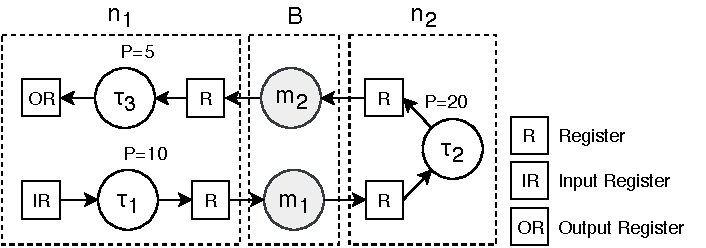
\includegraphics[width=0.7\linewidth]{img/cause_effect_chain_ntk}
	\caption{A Cause-effect Chain, mapped on nodes $n_1$ and $n_2$.}
	\label{fig_causeeffectchainntk}
\end{figure}
%\todo[inline]{better to cite this paper here: End-to-End Timing Analysis of Cause-Effect Chains in Automotive Embedded Systems}.

The end-to-end delay in a chain is the duration between the reading of data from the input register by the source task $Source(\sss{\Gamma})$ to the writing of same data to the output register by the last (or sink) task $Sink(\sss{\Gamma})$. Since we assume the chains consist of independently clocked tasks, the delay usually varies due to the undersampling and oversampling effects in the chains. In this work, we are particularly interested in the two types of delays that are widely used in the automotive and similar systems, namely the \textit{age delay} and the \textit{reaction delay}. 
\begin{figure}
	\centering
	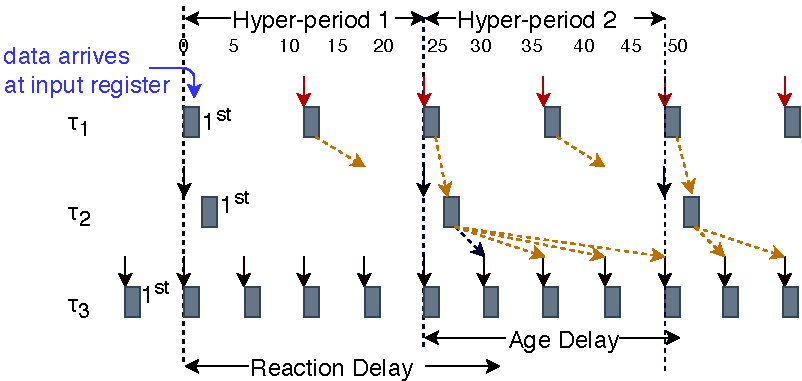
\includegraphics[width=0.9\linewidth]{img/timedchain_ntk}
	\caption{Reaction and Age Delays of the Cause-effect Chain, Shown in Figure {\ref{fig_causeeffectchainntk}}.}
	\label{fig_timedchainntk}
\end{figure}

The difference between the two types of delays is demonstrated in Figure~\ref{fig_timedpath}. The tasks $\tau_1$ and $\tau_2$ execute on node $n_1$, whereas task $\tau_3$ executes on node $n_2$. Note: $\tau_2$ communicates with $\tau_3$ via a CAN bus, which is not shown in the figure for simplicity. The red inverted arrows in the figure represent the reading of data from the input register, whereas the dashed-curve arrows represent the timed paths through which the data propagates from the input to the output of the chain. Thus, the age delay is the time elapsed between a stimulus and its corresponding latest non-overwritten response, i.e., between the $3^{rd}$ instance of  $\tau_1$  and the $10^{th}$ instance of $\tau_3$. It is frequently used in the control systems applications where freshness of data is paramount, e.g., braking a car over a bounded time. And, the reaction delay is the earliest time the system takes to respond to a stimulus that ``just missed" the read access at the input of the chain. Assume that data arrives just after the start of the $1^{st}$ instance of $\tau_1$ execution. The data corresponding to this event is not read by the current instance of $\tau_1$. In fact, the data will be read by the $2^{nd}$ instance of $\tau_1$. The earliest effect of this data at the output of the chain will appear at the $7^{th}$ instance of $\tau_3$, which represents the reaction delay. This delay is useful in the body-electronics domain where first reaction to events is important, e.g., in the button-to-reaction applications. For detailed discussion of the different delay semantics, we direct the reader to check research work by Mubeen et al.~\cite{mubeen2013support}. The age delay is computed using Equation (\ref{eqn_agedelay_singlenode}) and Equation (\ref{eqn_agedelay_multinode}) for a single node and multiple nodes, respectively.

\begin{align}
	\label{eqn_agedelay_singlenode}
	\Delta_{s}(\Gamma) &= \ssb{\alpha}[\tau_j]-\ssb{\alpha}[\tau_i] + \ssb{R}[\tau_j]&\text{single node}\\
	\label{eqn_agedelay_multinode}
	\Delta_{m}(\Gamma)&=\sum_{q\in subch(\Gamma)}{\Delta_s(q)} + \sum_{m\in msg(\Gamma)}{R_m}, &\text{muliple nodes}
\end{align}
where $\tau_j = sink(\Gamma)$, $\tau_i=source(\Gamma)$, $\alpha_\tau$ returns the activation time of $\tau$.

Assume $\Gamma \in \sss{\Gamma}$ is a chain, if the chain is mapped on a single node, the age delay $\Delta_s$ is a mere difference between the activation of the sink task $\ssb{\alpha}[\tau_j]$ and the activation of the source task $\ssb{\alpha}[\tau_i]$ plus the worst-case response time of the sink task $\ssb{R}[\tau_j]$ in the longest timed path that complies with the definition of the age delay. On the other hand, if the chain is mapped to multiple nodes, the age delay $\Delta_m$ can be compositionally computed~\cite{Feiertag2009ASemantics} as follows: the chain is partitioned  into a set of sub-chains per node, indicated by the predicate $subch(\Gamma)$, and for each sub-chain $a\in subch(\Gamma)$, the age delay is computed recursively using the same method to used to compute the age delay for a single node, and the result is added to the response-times of the messages involved in the chain, $msg(\Gamma)$.

\subsection{AUTOSAR Runnables}\label{subsec_autosarsystem}
The AUTOSAR standard introduced the notion of \textit{Runnables} to facilitate early analysis, that is at the VBF level, and to support interoperability of automotive applications across different execution platforms. Basically, runnables are schedulable pieces of codes similar to tasks. In this work, we assume periodically activated runnables with support for multiple worst-case executions that correspond to the different computation processor types. Unlike tasks, runnables' functional and extra-functional properties, e.g., timing, memory requirements, are part of the AUTOSAR software component specification. Therefore, the software application model defined in Definition~\ref{def_application} is extended to accommodate the notion of runnables, using the following simplified formal definition.

\begin{definition}[AUTOSAR Software Application Model]
It is modeled as directed acyclic vertex-weighted graph $g_r=\langle V_r, L_r, w_r, v\rangle$ of runnable nodes $V_r$, where $a_{ij}\in L_r$ represents either a triggering or data-flow link from the runnable $r_i$ to runnable $r_j$ and $i\neq j$. The cost $w_r=w$ defines the timing model of the runnable nodes, which is equivalently defined as the cost of the task nodes explained in Definition~\ref{def_application}.
\end{definition}

\begin{figure}[h!]
	\centering
	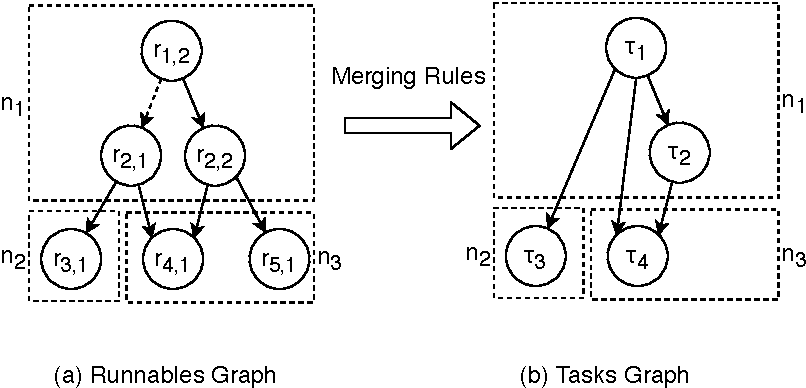
\includegraphics[width=0.7\linewidth]{img/runnable_task_dag}
	\caption[Example of a Software Application.]{Example of a Software Application, Modeled as Directed Acyclic Graph, where $\dashrightarrow$, $\dashrightarrow$ denote triggering link, data-flow link, respectively.}
	\label{fig_appexample}
\end{figure}

\begin{table}
	\parbox{.45\linewidth}{
		\centering
\begin{tabular}{|c|c|c|c|}
	\hline 
	\ttsss{r}[k][i,j] &$m_h$& $(e_h, P)$ & $\prec$ \ttsss{r} [k][i,j]\\ 
	\hline 
	1,1 & 1&$(1,10)$ & 2,1 \\ 
	\hline 
	2,1 &1& $(1,5)$ &  \\ 
	\hline 
	2,2 &1& $(1,15)$ &  \\ 
	\hline 
	3,1 & 2&$(1,20)$ &  \\ 
	\hline 
	4,1 & 3&$(1,10)$ &  \\ 
	\hline 
	5,1 & 3&$(1,20)$ &  \\ 
	\hline 
\end{tabular} 
		\caption{Runnables Timing Specifications.}
	}
	\hfill
	\parbox{.45\linewidth}{
		\centering
		\begin{tabular}{|c|c|c|}
			\hline 
			\ttsss{\tau} &$\bigcup\sss{r}[k][i,j]$& $(e_h,P)$ \\ 
			\hline 
			1 & 1,2;2,1 &  $(2,5)$\\ 
			\hline 
			2& 2,2 &  $(1,15)$\\ 
			\hline 
			3& 3,1 &  $(1,20)$\\ 
			\hline 
			4 & 4,1;5,1 &  $(1,10)$\\ 
			\hline 
		\end{tabular} 
		\caption{Tasks-Runnables Mappings.}
	}
\end{table}

According to the AUTOSAR specification \cite{AUTOSAR2017SpecificationSoftware}, runnables are mapped to tasks, and the tasks execute the runnables respecting their timing specifications. In the mapping process, one or more runnables can be merged to optimize the runtime execution by reducing the number of schedulable tasks. Thereore, through the mappings, eventually runnables graphs are refined by tasks graphs as shown in Figure{\ref{fig_appexample} (b). In this work, the following rules are applied in order to merge any runnables $a,b$, that is the link $(a, b)\in L_r$ merges to a task node $v\in V(g_\tau)$, if the following rules satisfy:
\begin{enumerate}[label=(\roman*)]
\item the runnables are co-hosted in the same computing node, that is \[a\mapsto m \land b\mapsto m\]
\item activation periods of the runnables are the same, i.e., $a.P = b.P$
\end{enumerate}

If the rules are satisfied, the task's timing specifications are set as follows: i) the WCET of the task is set to the sum of the WCET of the runnables, $v.e_i=a.e_i + b.e_i$, ii) the period and deadline of the task is  set to the least-common multiple (LCM) of the runnables' periods, $v.P=v.D=lcm(a.P, b.P)$. Otherwise, runnables are not merged, instead, each runnable that is not merged is mapped to a task while preserving the timing specifications of runnables.

% Following the grouping of runnables to tasks, We assume runnables communicate (or send data messages) at the end of the corresponding tasks' executions. The messages are packed into a single frame if destined to the same node otherwise each runnable communicats across a shared bus via a dedicated message entity, which is schedulable by the CAN bus controller. In essence, the assumed read-exec-write semantics of the runnables lowers the number of schedulable messages entities in the bus by facilitating packing of signals at the expense of restrictive (or less flexible) inter-runnables communication.

% Furthermore, we assume fixed and dynamic preemptive scheduling policies, that is each tasks sets allocated to a node must be schedulable according to the choice of the scheduling policy. For convenience, we assume priorities are assigned to tasks according to Rate Monotonic (RM) for the case of fixed scheduling policy, that is a task with a lower period get a higher priority.

%\subsection{Execution Platform}
%The execution platform provides computation and communication resources to the user applications, and is modeled as a \textit{complete} graph $\langle M,L^m\rangle$ of computation nodes, where $(m_i,m_j)\in L^m \land i\neq j$ refer to the communication links of the nodes, which are realized by a network bus, e.g., CAN. The computation nodes are heterogeneous with respect to parameters defined as a tuple $\langle hz, \lambda, p \rangle$, respectively denote processor speed, failure-rate and power consumption specifications. The allocation scheme is a mapping table $f:C\mapsto M$ from software components to computation nodes, where $C=\bigcup_{i=1}^{|A|} {V(A_i)}$ is the \textit{infinitary} union of the user applications' vertices, which denote nodes o software components.

\subsection{Reliability of Software Applications}\label{sub_reliability}
Redundancy is the most common way to increase the reliability of a system. In this context, \textit{software application reliability} refers to the probability that a software application functions correctly by the time $t$, or within the time interval $[0, t]$ \cite{Goel1985SoftwareApplicability}. Redandancy can be implemented according to different schemes, such as hot stand-by, cold stand-by, etc~\cite{Dubrova2013Fault-tolerantDesign}, in this work, we consider the hot-standby scheme, where replicated components maintain the same state. However, only the \textit{primary} replicas act on the environment, e.g., activating an actuator. The primary software component is the one in operation and is indicated by \ttsss{q}[k][i,1], the secondary software component, which is in the stand-by, by \ttsss{q}[k][i,2], etc., for a software application $A_k$.  Note: the software components are replicated unless the reliability requirements of applications are satisfied.

In this work the details of the redundancy scheme are abstracted away under the following assumptions: i) Hot stand-by redundancy technique is used for the replacement of failed components, which are identical and are allocated on different nodes, ii) software components need to be replicated if the application's reliability requirement is not met without replication, otherwise they are not replicated, iii) the time needed to detect and replace a faulty component is considered negligible and will not be taken into account in the response time analysis of tasks and delay calculation of cause-effect chains, iv) Because of its simplicity, the mechanism for detection and replacement of faulty components will be considered fault-free, and therefore will not be included in the reliability calculations.

Under this assumptions, the reliability of a software application is equivalent to the reliability of the execuiton platform such as the computating nodes and the communication bus, if any, on wich the application is deployed. The reliability of a computing node or the bus is calculated using $e^{\lambda t}$, where $\lambda$ is an exponentially distributed failure-rate. However, the reliability calcultion of the execution platform that services a software application is not trivial in the case with replication, e.g., the series-parallel reliability approach cannot be applied in the general case, due to the \textit{functional} interdependency created between computing nodes as the result. To demonstrate the functional interdependency, let us assume a software application $A_k$, having  component configurations with and without replication as shown Table \ref{fig_depwr} and \ref{fig_depwor}, respectively, where $\sss{q}[k][i,j]$ is the $j^{th}$ software-component replica of software-component type $\sss{c}\in \sss{C}$. Note: for readability of the example, we remove the superscript $k$.
\begin{figure}
	\begin{subfigure}{.5\textwidth}
		\centering
		\begin{tabular}{ccc}
			$n_1$ & $n_2$ & $n_3$\\
			\hline
			\ttssb{q}[1,1]&\ttssb{q}[2,1]& \\
			\ttssb{q}[3,1]& & \\
			\hline
		\end{tabular}	
		\caption{Without Replication.}
		\label{fig_depwor}
	\end{subfigure}%
	\begin{subfigure}{.5\textwidth}
		\centering
		\begin{tabular}{ccc}
			$n_1$ & $n_2$ & $n_3$\\
			\hline
			\ttssb{q}[1,1]&\ttssb{q}[2,1]& \ttssb{q}[2,2]\\
			\ttssb{q}[3,1]& \ttssb{q}[1,2]& \ttssb{q}[3,2]\\
			\hline
		\end{tabular}
		\caption{With Replication.}
		\label{fig_depwr}
	\end{subfigure}%
	\caption{Deployments of the Software Application $A_1$.}
	\label{fig_deployment}
\end{figure}

The reliability of the software application without replication forms a series path, indicated by the reliability block diagram (RBD) of Figure~\ref{fig_rbd}a, hence is computed as products of the reliability of $n_1,n_2$ and $B$. However, with replication, two computing nodes can form as series and parallel to service the sofware application,  e.g., due to \ttssb{q}[1,1] and \ttssb{q}[2,2] or \ttssb{q}[3,2], $n_1$ and $n_3$ make series, and due to \ttssb{q}[3,1] and \ttssb{q}[3,2], the nodes make parallel, to relialize partional functionality of the application. In this case, the series-parallel diagram depicted in Figure~\ref{fig_rbd}b does not accurately capture the reliaiblity calculation of the application with replication. Note: the red-dashed line between $n_1$ and $n_3$ indicates the possibility of the computing nodes becoming series. To address this problem, we use the exact reliability calculation technique based on the enumeration of the different failure states of the computing nodes, that is the different failure states of the execution platform is enumerated exaustively, and subsequently, the total probability the software application functions is computed, which is discussed in great length in Subsection~\ref{subsec_reliability_constraint}.
\begin{figure}
	\centering
	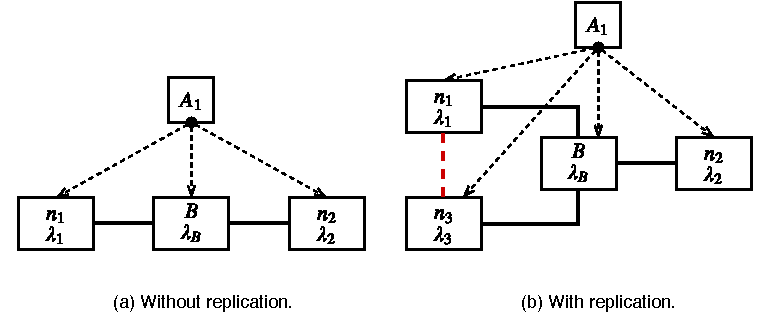
\includegraphics[width=0.8\linewidth]{img/rbd_replication}
	\caption{Reliability Block Diagrams of the Software Application.}
	\label{fig_rbd}
\end{figure}



